% Chapter 1

%\chapter{Curriculum Vitae} % Main chapter title

%\label{CV} % For referencing the chapter elsewhere, use \ref{Chapter1} 

% \lhead{Chapter 1. \emph{Introduction}} % This is for the header on each page - perhaps a shortened title
\pagenumbering{gobble}
\graphicspath{{./Pictures/}}

%\noindent\rule[0mm]{\linewidth}{2pt} old format
%----------------------------------------------------------------------------------------
\newgeometry{
  left=2cm,
  right=2.1cm,
  top=2cm,
  bottom=2cm,
  bindingoffset=5mm
}




\newpage
\pagestyle{plain}
\vspace{-9cm}

\huge
\textbf{Curriculum Vitae}

\bigskip
\bigskip
\large
\textbf{Personal Information}
\noindent\rule[3mm]{\linewidth}{1pt}

\normalsize
\vspace{-0.25cm}
\begin{tabbing}
First Name \hspace*{2.4cm} \= Raphael \\
Surname \> Wolfisberg \\
Date of Birth \> 14. May 1988 \\
Nationality \> Swiss \\
\medskip
E-mail \> raphael.w@hotmail.com \\
Mobile \> +41 (0) 79 837 19 62 
\end{tabbing}

\begin{addmargin}{0.03\textwidth}
\vspace{-4.1 cm}
\begin{flushright}
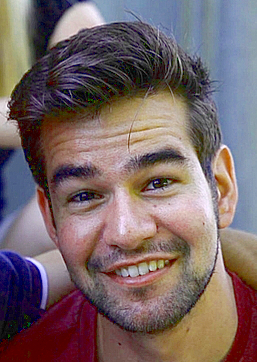
\includegraphics[scale=0.038]{Rafa} \\[1cm]
\end{flushright}
\end{addmargin}


\vspace{-0.7cm}
\large
\textbf{Education}
\noindent\rule[3mm]{\linewidth}{1pt}

\normalsize
\vspace{-0.7cm}
\begin{tabbing}
Mar. 2012 - present \hspace*{0.9cm} \= PhD in the Department of Chemistry and Biochemistry (DCB) \\ 
\> University of Bern, Switzerland  \\
\> Title of the PhD thesis: ``Characterization of the prelytic active \\ 
\> egress of a non-enveloped virus.'' \\
\> Supervisors: PD Dr. Carlos Ros and Prof. Dr. Christoph Kempf \\ [0.3cm]
Oct. - Dec. 2013 \> Scientific exchange at Centro de Biología Molecular Severo Ochoa \\
\> Universidad Autónoma de Madrid, Spain \\
\> Collaboration with Prof. Dr. José María Almendral del Río \\ [0.3cm]
Sept. 2010 - Jan. 2012 \> Master of Science (MSc) in Chemistry and Molecular Science \\
\> DCB, University of Bern, Switzerland  \\
\> Title of the master thesis: ``Changing the surface of human \\ \> parvovirus B19.'' \\
\> Supervisors: PD Dr. Carlos Ros and Prof. Dr. Christoph Kempf \\ [0.3cm]
Sept. 2007 - Aug. 2010 \> Bachelor of Science (BSc) in Chemistry or Biochemistry \\
\> DCB, University of Bern, Switzerland  \\
\> Title of the bachelor thesis: ``Die Suche nach dem NMD \\
\> Mechanismus in \textit{Trypanosoma brucei}.'' \\
\> Supervisor: Prof. Dr. André Schneider
\end{tabbing}

\vspace{0.2 cm}
\large
\textbf{Teaching experience}
\noindent\rule[3mm]{\linewidth}{1pt}

\normalsize
\vspace{-0.2cm}
Teaching of undergraduate students in biochemistry internships at the University of Bern.

\vspace{0.475 cm}
\large
\textbf{Conferences}
\noindent\rule[3mm]{\linewidth}{1pt}

\normalsize
\vspace{-0.6 cm}
\begin{tabbing}
22.-26. June 2014 \hspace{1.27 cm} \= 15\textsuperscript{th} Biennial International Parvovirus Workshop \hspace{0.1 cm} \= Bordeaux, France
\end{tabbing}



\clearpage

\large
\textbf{Publications}
\noindent\rule[3mm]{\linewidth}{1pt}

\normalsize


\vspace{-0.25cm}
\textbf{\emph{Peer-reviewed journal articles}} \\[0.3 cm]

\begin{addmargin}{0.025\textwidth}
\textbf{Wolfisberg R}, Ruprecht N, Kempf C, Ros C. Impaired genome encapsidation
restricts the \\
\textit{in vitro} propagation of human parvovirus B19. \\
\textit{J Virol Methods.} 2013 Oct;193(1):215-25. \\[0.3 cm]

\textbf{Wolfisberg R}, Kempf C, Ros C. Late maturation steps in the nucleus preceding prelytic\\
 active egress of a non-enveloped parvovirus.\\ 
 \textit{Manuscript in preparation}
\end{addmargin}


\vspace{0.275 cm}
\large
\textbf{Skills}
\noindent\rule[3mm]{\linewidth}{1pt}

\normalsize
\vspace{-0.5 cm}
\begin{tabbing}
Languages \hspace{2.879 cm} \= German (Mother tongue), English (Advanced), \\
\> French (Intermediate level), Spanish (Basic knowledge) \\ [0.15 cm]
Operating Systems \> Microsoft Windows, Apple OS X \\ [0.15cm]
Programs \> Typesetting (Apple iWork, \LaTeX, Microsoft Office) \\
\> Molecular modeling (PyMOL, UCSF Chimera)\\
\> Data processing (GraphPad Prism, Mathcad)
\end{tabbing}




%\Large
%\textbf{Memberships}
%\noindent\rule[4mm]{\linewidth}{1pt}

%\normalsize
%\vspace{-0.5cm}
%\vspace{0.2 cm}
%Swiss Society for Molecular and Cellular Biosciences (SSMCB)

\vspace{0.275 cm}

\large
\textbf{Other activities}
\noindent\rule[3mm]{\linewidth}{1pt}

\normalsize
\vspace{-0.25cm}
Organizing and supervising holidays for physically and mentally handicapped persons with Insieme Luzern in collaboration with the Swiss civil defense.
\vspace{-0.1 cm}
\begin{tabbing}
Accordion \=(Handharmonikaorchester Solothurn) \\[0.15 cm]
Athletics \>(KTV Neuenkirch) 
\end{tabbing}



\vspace{0.475 cm}
\large
\textbf{References}
\noindent\rule[3mm]{\linewidth}{1pt}

 
\vspace{-0.5 cm}
\begin{tabbing}
PD Dr. Carlos Ros \hspace{5.4 cm} \= Prof. Dr. Christoph Kempf \\
Department of Chemistry and Biochemistry \> Department of Chemistry and Biochemistry \\
University of Bern \> University of Bern \\
Freiestrasse 3, 3012 Bern \> Freiestrasse 3, 3012 Bern \\
Switzerland \> Switzerland \\ [0.1 cm]
+41 (0) 31 631 43 49 \> +41 (0) 31 631 43 31\\ [0.55 cm]

Prof. Dr. José María Almendral del Río \\
Centro de Biología Molecular Severo Ochoa \\
Universidad Autónoma de Madrid \\
Cantoblanco, \np{28049} Madrid \\
Spain \\ [0.1 cm]
+34 (0) 91 196 45 59






\end{tabbing}

\restoregeometry
\pagenumbering{arabic}